\begin{standout}[第三章]
    非线性结构\\
    Non-Linear Structures
\end{standout}

\begin{frame}{大纲}
    \setbeamertemplate{section in toc}[sections numbered]
    % \begin{multicols}{2}
    \tableofcontents
    % \end{multicols}
\end{frame}

\begin{fragile}
    \bicolumns[0.6]{
        \begin{exampleblock}{引例:Königsberg七桥问题}
            \begin{itemize}
                \item 在Königsberg市有$7$座桥连通了$4$块区域
                \item 是否有算法实现
                      \begin{itemize}
                          \item 从某处出发
                          \item 依次穿过所有桥仅$1$次
                          \item 回到原地
                      \end{itemize}
                \item<2> 可抽象为图的一笔画问题
            \end{itemize}
        \end{exampleblock}
    }{
        \begin{figure}
            \centering
            \only<1>{
                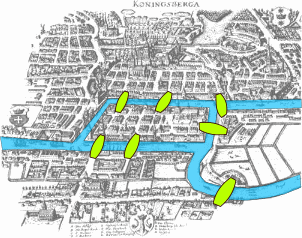
\includegraphics[height=3.6cm]{images/Konigsberg_bridges.png}
            }
            \only<2>{
                \begin{tikzpicture}[ >=stealth, thick, black!50, %
                        list item/.style={draw=gray, circle, thick}, %
                    ]
                    \node (a) [terminal] at (-2,0) {$A$};
                    \node (b) [terminal] at (0,-1.5) {$B$};
                    \node (c) [terminal] at (2,0) {$C$};
                    \node (d) [terminal] at (0,1.5) {$D$};
                    \draw (a) to [bend left] (b);
                    \draw (a) to [bend right] (b);
                    \draw (a) to [bend left] (d);
                    \draw (a) to [bend right] (d);
                    \draw (b) to [bend right] (c);
                    \draw (d) to [bend left] (c);
                    \draw (a) to (c);
                \end{tikzpicture}
            }
            \caption{Königsberg七桥问题}
            \label{fig:demo-Königsberg}
        \end{figure}
    }
\end{fragile}

\begin{frame}
    \begin{block}{非线性结构}
        \begin{itemize}
            \item 在半线性结构的基础上允许有环的存在
            \item 半线性结构的一种扩展
            \item 非线性结构主要指\textbf{图}结构
            \item 图与树之间可转换
        \end{itemize}
    \end{block}
\end{frame}

\section{基本术语}

\begin{fragile}
    \frametitle{\insertsectionhead}
    \bicolumns[0.5]{
        \begin{block}{图(Graph)}
            \begin{itemize}
                \item 可被定义为$G=(V,E)$,其中\footnotemark
                      \begin{itemize}
                          \item 集合$V$中元素$v$为\textbf{顶点(vertex)}
                          \item 集合$E$中元素$e\in{V}\times{V}$为\textbf{边
                                    (edge)}
                      \end{itemize}
                \item 只定义\alert{拓扑}关系,与几何位置无关
            \end{itemize}
        \end{block}
    }{
        \begin{figure}
            \centering
            \begin{tikzpicture}[ >=stealth, thick, black!50, %
                    list item/.style={draw=gray, circle, thick}, %
                ]
                \node (a) [terminal] at (-2,0) {$v_{0}$};
                \node (b) [terminal] at (0,-1.5) {$v_{1}$};
                \node (c) [terminal] at (2,0) {$v_{2}$};
                \node (d) [terminal] at (0,1.5) {$v_{3}$};
                \draw[->] (a) to [bend left] node [pos=0.7,above,sloped] {$e_{0}$} (b);
                \draw[<-] (a) to [bend right] node [pos=0.5,below,sloped] {$e_{1}$} (b);
                \draw[->] (a) to [bend left] node [pos=0.5,above,sloped] {$e_{2}$} (d);
                \draw[<-] (a) to [bend right] node [pos=0.7,below,sloped] {$e_{3}$} (d);
                \draw (b) to [bend right] node [pos=0.5,below,sloped] {$e_{4}$} (c);
                \draw (d) to [bend left] node [pos=0.5,above,sloped] {$e_{5}$} (c);
                \draw (a) to node [pos=0.7,above,sloped] {$e_{6}$} (c);
            \end{tikzpicture}
            \caption{图}
            \label{fig:demo-graph}
        \end{figure}
    }

    \footnotetext{顶点又名\textbf{结点(node)},边又名\textbf{弧(arc)},且$V$与
        $E$均为有限集}
\end{fragile}

\begin{fragile}
    \frametitle{\insertsectionhead}
    \bicolumns[0.5]{
        \begin{block}{无向图(Undigraph)与有向图(Digraph)}
            \begin{itemize}
                \item 按顶点是否有顺序可将边$e$分为
                      \begin{itemize}
                          \item 无顺序的\textbf{无向边},记作$(u,v)$
                          \item 有顺序的\textbf{有向边},记作
                                $\langle{u,v}\rangle$
                      \end{itemize}
                \item 只有无向边的图为\textbf{无向图}
                \item 只有有向边的图为\textbf{有向图}
                \item 二者均有的图为\textbf{混合图(mixed graph)}
                \item 无向图与混合图均可转化为有向图
                      \begin{itemize}
                          \item 将一条无向边拆成两条相反的有向边
                      \end{itemize}
            \end{itemize}
        \end{block}
    }{
        \begin{figure}
            \centering
            \begin{subfigure}[T]{0.9\textwidth}
                \centering
                \begin{tikzpicture}[ >=stealth, thick, black!50, %
                        list item/.style={draw=gray, circle, thick}, %
                    ]
                    \node (a) [terminal] at (-2,0) {$v_{0}$};
                    \node (b) [terminal] at (0,-.5) {$v_{1}$};
                    \node (c) [terminal] at (2,0) {$v_{2}$};
                    \node (d) [terminal] at (0,.5) {$v_{3}$};
                    \draw[->] (a) to (b);
                    \draw[<-] (a) to (d);
                    \draw[->] (b) to (c);
                    \draw[->] (d) to (c);
                    \draw[->] (a) to (c);
                \end{tikzpicture}
                \caption{有向图}
                \label{subfig:digraph}
            \end{subfigure}
            ~
            \begin{subfigure}[T]{0.9\textwidth}
                \centering
                \begin{tikzpicture}[ >=stealth, thick, black!50, %
                        list item/.style={draw=gray, circle, thick}, %
                    ]
                    \node (a) [terminal] at (-2,0) {$v_{0}$};
                    \node (b) [terminal] at (0,-.5) {$v_{1}$};
                    \node (c) [terminal] at (2,0) {$v_{2}$};
                    \node (d) [terminal] at (0,.5) {$v_{3}$};
                    \draw (a) to (b);
                    \draw (a) to (d);
                    \draw (b) to (c);
                    \draw (d) to (c);
                    \draw (a) to (c);
                \end{tikzpicture}
                \caption{无向图}
                \label{subfig:undigraph}
            \end{subfigure}
            \caption{有向图与无向图}
            \label{fig:digraph_undigraph}
        \end{figure}
    }
\end{fragile}

\begin{fragile}
    \frametitle{\insertsectionhead}
    \bicolumns[0.55]{
        \begin{block}{顶点的度(Degree)}
            \begin{itemize}
                \item 若边$e=\langle{}v_{a},v_{b}\rangle$,则
                      \begin{itemize}
                          \item 称$v_{a}$与$v_{b}$\textbf{邻接(adjacent)}
                          \item 称二者均与$e$彼此\textbf{关联(incident)}
                          \item 称$e$为$v_{a}$的\textbf{出边(outgoing edge)}
                          \item 称$e$为$v_{b}$的\textbf{入边(incoming edge)}
                      \end{itemize}
                \item 在无向图中称与顶点$v$关联的边数为$v$的\textbf{度}
                \item 在有向图中称与顶点$v$关联的出入边数分别为$v$的\textbf{出
                          度(out-degree)}与\textbf{入度(in-degree)}
            \end{itemize}
        \end{block}
    }{
        \begin{figure}
            \centering
            \begin{subfigure}[T]{0.9\textwidth}
                \centering
                \begin{tikzpicture}[ >=stealth, thick, black!50, %
                        list item/.style={draw=gray, circle, thick}, %
                        every node/.style={terminal, rectangle split, rectangle split horizontal, rectangle split parts=2}, %
                    ]
                    \node (a) at (-1.5,0) {$2$\nodepart{two}$1$};
                    \node (b) at (0,-.5) {$1$\nodepart{two}$1$};
                    \node (c) at (1.5,0) {$0$\nodepart{two}$3$};
                    \node (d) at (0,.5) {$1$\nodepart{two}$1$};
                    \draw[->] (a) to (b);
                    \draw[<-] (a) to (d);
                    \draw[->] (b) to (c);
                    \draw[->] (d) to (c);
                    \draw[->] (a) to (c);
                \end{tikzpicture}
                \caption{有向图的出度(左)与入度(右)}
                \label{subfig:degree_digraph}
            \end{subfigure}
            ~
            \begin{subfigure}[T]{0.9\textwidth}
                \centering
                \begin{tikzpicture}[ >=stealth, thick, black!50, %
                        list item/.style={draw=gray, circle, thick}, %
                    ]
                    \node (a) [terminal] at (-1.5,0) {$3$};
                    \node (b) [terminal] at (0,-.5) {$2$};
                    \node (c) [terminal] at (1.5,0) {$3$};
                    \node (d) [terminal] at (0,.5) {$2$};
                    \draw (a) to (b);
                    \draw (a) to (d);
                    \draw (b) to (c);
                    \draw (d) to (c);
                    \draw (a) to (c);
                \end{tikzpicture}
                \caption{无向图的度}
                \label{subfig:degree_undigraph}
            \end{subfigure}
            \caption{顶点的度}
            \label{fig:degree_digraph_undigraph}
        \end{figure}
    }
\end{fragile}

\begin{frame}
    \frametitle{\insertsectionhead}
    \begin{block}{简单图(Simple Graph)}
        \begin{itemize}
            \item 称起点与终点相同的边为\textbf{自环(self-loop)}
            \item 称\alert{不含}自环且所有边均\alert{唯一}的图为\textbf{简单
                      图}\footnote{本课程只讨论简单图}
        \end{itemize}
    \end{block}
    \begin{figure}
        \centering
        \begin{subfigure}[T]{0.3\textwidth}
            \centering
            \begin{tikzpicture}[ >=stealth, thick, black!50, %
                    list item/.style={draw=gray, circle, thick}, %
                ]
                \node (a) [terminal] at (-1.5,0) {$v_{0}$};
                \node (b) [terminal] at (0,-.5) {$v_{1}$};
                \node (c) [terminal] at (1.5,0) {$v_{2}$};
                \node (d) [terminal] at (0,.5) {$v_{3}$};
                \draw (a) to (b);
                \draw (a) to (d);
                \draw (b) to (c);
                \draw (d) to (c);
                \draw (a) to (c);
            \end{tikzpicture}
            \caption{简单图}
            \label{subfig:simple_graph}
        \end{subfigure}
        ~
        \begin{subfigure}[T]{0.3\textwidth}
            \centering
            \begin{tikzpicture}[ >=stealth, thick, black!50, %
                    list item/.style={draw=gray, circle, thick}, %
                ]
                \node (a) [terminal] at (-1.5,0) {$v_{0}$};
                \node (b) [terminal] at (0,-.5) {$v_{1}$};
                \node (c) [terminal] at (1.5,0) {$v_{2}$};
                \node (d) [terminal] at (0,.5) {$v_{3}$};
                \draw (a) to (b);
                \draw[red] (a) to [loop above] ();
                \draw (a) to (d);
                \draw (b) to (c);
                \draw (d) to (c);
                \draw (a) to (c);
            \end{tikzpicture}
            \caption{带自环的非简单图}
            \label{subfig:non_simple_graph_a}
        \end{subfigure}
        ~
        \begin{subfigure}[T]{0.3\textwidth}
            \centering
            \begin{tikzpicture}[ >=stealth, thick, black!50, %
                    list item/.style={draw=gray, circle, thick}, %
                ]
                \node (a) [terminal] at (-1.5,0) {$v_{0}$};
                \node (b) [terminal] at (0,-.5) {$v_{1}$};
                \node (c) [terminal] at (1.5,0) {$v_{2}$};
                \node (d) [terminal] at (0,.5) {$v_{3}$};
                \draw (a) to (b);
                \draw[red] (a) to [bend right] (b);
                \draw (a) to (d);
                \draw (b) to (c);
                \draw (d) to (c);
                \draw (a) to (c);
            \end{tikzpicture}
            \caption{有重复边的非简单图}
            \label{subfig:non_simple_graph_b}
        \end{subfigure}
        \caption{简单图与非简单图}
        \label{fig:simple_graph_non_simple_graph}
    \end{figure}
\end{frame}

\begin{fragile}
    \frametitle{\insertsectionhead}
    \begin{block}{路径(Path)}
        \begin{itemize}
            \item 若序列$\pi=\{v_{k}\}_{k=0}^{n}$满足$v_{k}$与$v_{k+1}$\alert{邻
                      接}\footnote{指存在边$e_{k}$满足$e_{k}=(v_{k},v_{k+1})$或
                  $e_{k}=\langle{}v_{k},v_{k+1}\rangle$,$k\in\mathbb{Z}\cap[0,n)$},
                  则称之为自$v_{0}$至$v_{n}$的一条\textbf{路径}
                  \begin{itemize}
                      \item 称经过的总边数$|\pi|-1$为路径\textbf{长度(length)}
                      \item 称无重复顶点的路径为\textbf{简单(simple)路径}
                  \end{itemize}
            \item 两顶点间的路径一般\alert{不唯一}
        \end{itemize}
    \end{block}
    \begin{figure}
        \centering
        \begin{subfigure}[T]{0.3\textwidth}
            \centering
            \begin{tikzpicture}[ >=stealth, thick, black!50, %
                    list item/.style={draw=gray, circle, thick}, %
                ]
                \node (a) [terminal] at (-1.5,0) {$v_{0}$};
                \node (b) [terminal] at (0,-.5) {$v_{1}$};
                \node (c) [terminal] at (1.5,0) {$v_{2}$};
                \node (d) [terminal] at (0,.5) {$v_{3}$};
                \draw[<-,red] (a) to (b);
                \draw (a) to (d);
                \draw (b) to (c);
                \draw[<-,red] (d) to (c);
                \draw[->,red] (a) to (c);
            \end{tikzpicture}
            \caption{简单路径:$(v_{1},v_{0},v_{2},v_{3})$}
            \label{subfig:simple_path}
        \end{subfigure}
        ~
        \begin{subfigure}[T]{0.3\textwidth}
            \centering
            \begin{tikzpicture}[ >=stealth, thick, black!50, %
                    list item/.style={draw=gray, circle, thick}, %
                ]
                \node (a) [terminal] at (-1.5,0) {$v_{0}$};
                \node (b) [terminal] at (0,-.5) {$v_{1}$};
                \node (c) [terminal] at (1.5,0) {$v_{2}$};
                \node (d) [terminal] at (0,.5) {$v_{3}$};
                \draw[<-,red] (a) to (b);
                \draw[<-,red] (a) to (d);
                \draw (b) to (c);
                \draw[<-,red] (d) to (c);
                \draw[->,red] (a) to (c);
            \end{tikzpicture}
            \caption{非简单路径:$(v_{1},v_{0},v_{2},v_{3},v_{0})$}
            \label{subfig:non_simple_path}
        \end{subfigure}
        \caption{图的路径}
        \label{fig:graph_paths}
    \end{figure}
\end{fragile}

\begin{fragile}
    \frametitle{\insertsectionhead}
    \begin{block}{环路(Cycle)}
        \begin{itemize}
            \item 若路径$\pi=\{v_{k}\}_{k=0}^{n}$中起止顶点相同,即
                  $v_{0}=v_{n}$,则称其为\textbf{环路}
                  \begin{itemize}
                      \item 若除起止顶点相同外无任何其他顶点两两相同,则称其为
                            \textbf{简单环路}
                      \item 称经过图中各\alert{边}一次且仅一次的环路为\textbf{欧
                                拉环路(Eulerian tour)}
                      \item 称经过图中各\alert{顶点}一次且仅一次的环路为
                            \textbf{哈米尔顿环路(Hamiltonian tour)}
                  \end{itemize}
        \end{itemize}
    \end{block}
    \begin{figure}
        \centering
        \begin{subfigure}[T]{0.3\textwidth}
            \centering
            \begin{tikzpicture}[ >=stealth, thick, black!50, %
                    list item/.style={draw=gray, circle, thick}, %
                ]
                \node (a) [terminal] at (-1.5,0) {$v_{0}$};
                \node (b) [terminal] at (0,-.5) {$v_{1}$};
                \node (c) [terminal] at (1.5,0) {$v_{2}$};
                \node (d) [terminal] at (0,.5) {$v_{3}$};
                \draw[->] (a) to (b);
                \draw[<-,red] (a) to (d);
                \draw[->] (b) to (c);
                \draw[<-,red] (d) to (c);
                \draw[->,red] (a) to (c);
                \draw[<-] (a) to [bend left=60] (c);
            \end{tikzpicture}
            \caption{简单环路:$(v_{0},v_{2},v_{3})$}
            \label{subfig:simple_cycle}
        \end{subfigure}
        \begin{subfigure}[T]{0.35\textwidth}
            \centering
            \begin{tikzpicture}[ >=stealth, thick, black!50, %
                    list item/.style={draw=gray, circle, thick}, %
                ]
                \node (a) [terminal] at (-1.5,0) {$v_{0}$};
                \node (b) [terminal] at (0,-.5) {$v_{1}$};
                \node (c) [terminal] at (1.5,0) {$v_{2}$};
                \node (d) [terminal] at (0,.5) {$v_{3}$};
                \draw[->,red] (a) to (b);
                \draw[<-,red] (a) to (d);
                \draw[->,red] (b) to (c);
                \draw[<-,red] (d) to (c);
                \draw[->,red] (a) to (c);
                \draw[<-,red] (a) to [bend left=60] (c);
            \end{tikzpicture}
            \caption{欧拉环路:$(v_{0},v_{1},v_{2},v_{0},v_{2},v_{3},v_{0})$}
            \label{subfig:demo_euler_tour}
        \end{subfigure}
        \begin{subfigure}[T]{0.32\textwidth}
            \centering
            \begin{tikzpicture}[ >=stealth, thick, black!50, %
                    list item/.style={draw=gray, circle, thick}, %
                ]
                \node (a) [terminal] at (-1.5,0) {$v_{0}$};
                \node (b) [terminal] at (0,-.5) {$v_{1}$};
                \node (c) [terminal] at (1.5,0) {$v_{2}$};
                \node (d) [terminal] at (0,.5) {$v_{3}$};
                \draw[->,red] (a) to (b);
                \draw[<-,red] (a) to (d);
                \draw[->,red] (b) to (c);
                \draw[<-,red] (d) to (c);
                \draw[->] (a) to (c);
                \draw[<-] (a) to [bend left=60] (c);
            \end{tikzpicture}
            \caption{哈米尔顿环路:$(v_{0},v_{1},v_{2},v_{3},v_{0})$}
            \label{subfig:demo_hamiltonian_tour}
        \end{subfigure}
        \caption{图的环路}
        \label{fig:graph_cycles}
    \end{figure}
\end{fragile}

\begin{fragile}
    \frametitle{\insertsectionhead}
    \begin{block}{完全图(Complete Graph)}
        \begin{itemize}
            \item 图中任意两顶点均邻接
            \item 若顶点数为$n$则无向与有向边数分别为$\frac{n(n-1)}{2}$与
            $n(n-1)$
        \end{itemize}
    \end{block}
    \begin{figure}
        \centering
        \begin{subfigure}[b]{0.3\textwidth}
            \centering
            \begin{tikzpicture}[ >=stealth, thick, black!50, %
                    list item/.style={draw=gray, circle, thick}, %
                ]
                \node (a) [terminal] at (-1.5,0) {$v_{0}$};
                \node (b) [terminal] at (0,-0.75) {$v_{1}$};
                \node (c) [terminal] at (1.5,0) {$v_{2}$};
                \node (d) [terminal] at (0,0.75) {$v_{3}$};
                \draw (a) to (b);
                \draw (a) to [bend right=90] (c);
                \draw (a) to (d);
                \draw (b) to (c);
                \draw (b) to (d);
                \draw (c) to (d);
            \end{tikzpicture}
            \caption{完全无向图}
            \label{subfig:complete_undigraph}
        \end{subfigure}
        ~
        \begin{subfigure}[b]{0.3\textwidth}
            \centering
            \begin{tikzpicture}[ >=stealth, thick, black!50, %
                    list item/.style={draw=gray, circle, thick}, %
                ]
                \node (a) [terminal] at (-1.5,0) {$v_{0}$};
                \node (b) [terminal] at (0,-0.75) {$v_{1}$};
                \node (c) [terminal] at (1.5,0) {$v_{2}$};
                \node (d) [terminal] at (0,0.75) {$v_{3}$};
                \draw[->] (a) to [bend right=10] (b);
                \draw[->] (a) to [bend right=90] (c);
                \draw[->] (a) to [bend right=10] (d);
                \draw[->] (b) to [bend right=10] (c);
                \draw[->] (b) to [bend right=10] (d);
                \draw[->] (c) to [bend right=10] (d);
                \draw[<-] (a) to [bend left=10] (b);
                \draw[<-] (a) to [bend left=90] (c);
                \draw[<-] (a) to [bend left=10] (d);
                \draw[<-] (b) to [bend left=10] (c);
                \draw[<-] (b) to [bend left=10] (d);
                \draw[<-] (c) to [bend left=10] (d);
            \end{tikzpicture}
            \caption{完全有向图}
            \label{subfig:demo_complete_digraph}
        \end{subfigure}
        \caption{完全图}
        \label{fig:complete_graphs}
    \end{figure}
\end{fragile}

\begin{fragile}
    \frametitle{\insertsectionhead}
    \begin{block}{带权图(Weighted Graph)}
        \begin{itemize}
            \item 为每条边指定权重,又名\textbf{带权网络(network)}
            \item 用于表示顶点关系的细节,如长度、流量、成本等
            \item 普通图可看作所有边权重均为$1$的带权图
        \end{itemize}
    \end{block}
    \begin{figure}
        \centering
        \begin{subfigure}[T]{0.3\textwidth}
            \centering
            \begin{tikzpicture}[ >=stealth, thick, black!50, %
                    list item/.style={draw=gray, circle, thick}, %
                ]
                \node (a) [terminal] at (-1.5,0) {$v_{0}$};
                \node (b) [terminal] at (0,-.5) {$v_{1}$};
                \node (c) [terminal] at (1.5,0) {$v_{2}$};
                \node (d) [terminal] at (0,.5) {$v_{3}$};
                \draw[->] (a) to (b);
                \draw[<-] (a) to (d);
                \draw[->] (b) to (c);
                \draw[<-] (d) to (c);
                \draw[->] (a) to (c);
            \end{tikzpicture}
            \caption{普通图}
            \label{subfig:non_weighted_graph}
        \end{subfigure}
        ~
        \begin{subfigure}[T]{0.3\textwidth}
            \centering
            \begin{tikzpicture}[ >=stealth, thick, black!50, %
                    list item/.style={draw=gray, circle, thick}, %
                ]
                \node (a) [terminal] at (-1.5,0) {$v_{0}$};
                \node (b) [terminal] at (0,-.5) {$v_{1}$};
                \node (c) [terminal] at (1.5,0) {$v_{2}$};
                \node (d) [terminal] at (0,.5) {$v_{3}$};
                \draw[->] (a) to node [pos=0.5,below,sloped] {$w_{0}$} (b);
                \draw[<-] (a) to node [pos=0.5,above,sloped] {$w_{1}$} (d);
                \draw[->] (b) to node [pos=0.5,below,sloped] {$w_{2}$} (c);
                \draw[<-] (d) to node [pos=0.5,above,sloped] {$w_{3}$} (c);
                \draw[->] (a) to node [pos=0.5,sloped] {$w_{4}$} (c);
            \end{tikzpicture}
            \caption{带权图}
            \label{subfig:demo_weighted_graph}
        \end{subfigure}
        \caption{普通图与带权图}
        \label{fig:weighted_graphs}
    \end{figure}
\end{fragile}
\section{图的存储结构}

\begin{fragile}
    \frametitle{\insertsectionhead}
    \begin{block}{图的抽象数据类型}
        \begin{minted}[linenos=false,escapeinside=@@]{c}
            ADT Graph {
            数据:
                数据对象: @$\mathcal{D} = \{v_{k} | v_{k}\in\text{顶点集合}, k\in\mathbb{Z}\cap[1,n]\}$@
                逻辑关系: @$\mathcal{R} = \{\langle{}v_{x},v_{y}\rangle | \exists{e_{x}}\in\text{边集合}, s.t.\;e_{x}=\langle{}v_{x},v_{y}\rangle\}$@
            操作:
                create_graph(), destroy_graph(g)
                    构造与销毁一个图@$g$@
                get_vertex(g, v), get_first_neighbor(g, v), get_next_neighbor(g, v, w)
                    返回顶点@$v$@的信息, 获取顶点@$v$@的第一个邻接顶点与相对于@$w$@的下一个邻接顶点
                insert_vertex(g, v), remove_vertex(g, v)
                    插入与删除顶点@$v$@
                insert_edge(g, va, vb), remove_edge(g, va, vb)
                    在顶点@$v_{a}$@与@$v_{b}$@间插入与删除一条边
                depth_first_search(g, x), breadth_first_search(g, x)
                    对图@$g$@进行深度与广度优先搜索值@$x$@
            }
        \end{minted}
    \end{block}
\end{fragile}

\begin{fragile}
    \frametitle{\insertsectionhead}
    \begin{block}{邻接矩阵(Adjacency Matrix)}
        \begin{itemize}
            \item 图抽象数据类型的一种基本实现
            \item 用稠密方阵表示,其元素描述一对顶点间可能的邻接关系
                  \begin{itemize}
                      \item 若有边相连,则元素为该边权重;否则可为$\infty$或$0$
                  \end{itemize}
        \end{itemize}
    \end{block}
    \vspace{-4ex}
    \begin{figure}
        \centering
        \begin{subfigure}[b]{0.45\textwidth}
            \centering
            \begin{tikzpicture}[ >=stealth, thick, black!50, %
                    list item/.style={draw=gray, circle, thick}, %
                ]
                \node (a) [terminal] at (-1.5,0) {$v_{0}$};
                \node (b) [terminal] at (0,-.5) {$v_{1}$};
                \node (c) [terminal] at (1.5,0) {$v_{2}$};
                \node (d) [terminal] at (0,.5) {$v_{3}$};
                \draw[->] (a) to node [pos=0.5,below,sloped] {$w_{0}$} (b);
                \draw[<-] (a) to node [pos=0.5,above,sloped] {$w_{1}$} (d);
                \draw[->] (b) to node [pos=0.5,below,sloped] {$w_{2}$} (c);
                \draw[<-] (d) to node [pos=0.5,above,sloped] {$w_{3}$} (c);
                \draw[->] (a) to node [pos=0.5,sloped] {$w_{4}$} (c);
            \end{tikzpicture}
            \caption{带权图}
            \label{subfig:demo__weighted_graph}
        \end{subfigure}
        \begin{subfigure}[b]{0.45\textwidth}
            \centering
            \[
                \bordermatrix{ ~ & v_{0} & v_{1} & v_{2} & v_{3} \cr
                    v_{0} & \infty & w_{0}  & w_{4}  & \infty \cr
                    v_{1} & \infty & \infty & w_{2}  & \infty \cr
                    v_{2} & \infty & \infty & \infty & w_{3}  \cr
                    v_{3} & w_{1}  & \infty & \infty & \infty \cr}
            \]\vspace{-2ex}
            \caption{带权图的邻接矩阵}
            \label{subfig:demo__adjacent_matrix}
        \end{subfigure}
        \caption{邻接矩阵}
        \label{fig:demo_adjacent_matrix}
    \end{figure}
\end{fragile}

\begin{frame}
    \frametitle{\insertsectionhead}
    \begin{exampleblock}{邻接矩阵特点}
        \begin{itemize}
            \item 无向图邻接矩阵必\alert{对称},故可只存储上三角部分
            \item 有向图邻接矩阵第$k$\alert{行/列}非零元素个数为对应顶点的
                  \alert{出/入度}
            \item 增删边只需修改矩阵特定元素值
            \item 增删顶点需调整矩阵\alert{维度},导致大量元素移动
        \end{itemize}
    \end{exampleblock}
    \begin{exampleblock}{复杂度}
        \begin{itemize}
            \item 空间复杂度:$O(n^{2})$,不利于表达\alert{稀疏图(sparse
                      graph)\footnote{指边数远小于完全图边数的图}}
            \item 查找特定边的时间复杂度:$O(1)$
        \end{itemize}
    \end{exampleblock}
\end{frame}

\begin{fragile}
    \frametitle{\insertsectionhead}
    \begin{block}{邻接表(Adjacency List)}
        \begin{itemize}
            \item 每个顶点以\alert{链表}存储其邻接顶点集合
                  \begin{itemize}
                      \item 链表结点存储信息包括:顶点序号、边权重、下一个邻接顶
                            点
                  \end{itemize}
            \item 相当于只存储邻接矩阵中的有效元素
        \end{itemize}
    \end{block}
    % \vspace{-4ex}
    \begin{figure}
        \centering
        \begin{subfigure}[b]{0.45\textwidth}
            \centering
            \begin{tikzpicture}[ >=stealth, thick, black!50, %
                    list item/.style={draw=gray, circle, thick}, %
                ]
                \node (a) [terminal] at (-1.5,0) {$v_{0}$};
                \node (b) [terminal] at (0,-.5) {$v_{1}$};
                \node (c) [terminal] at (1.5,0) {$v_{2}$};
                \node (d) [terminal] at (0,.5) {$v_{3}$};
                \draw[->] (a) to node [pos=0.5,below,sloped] {$w_{0}$} (b);
                \draw[<-] (a) to node [pos=0.5,above,sloped] {$w_{1}$} (d);
                \draw[->] (b) to node [pos=0.5,below,sloped] {$w_{2}$} (c);
                \draw[<-] (d) to node [pos=0.5,above,sloped] {$w_{3}$} (c);
                \draw[->] (a) to node [pos=0.5,sloped] {$w_{4}$} (c);
            \end{tikzpicture}
            \caption{带权图}
            \label{subfig:demo___weighted_graph}
        \end{subfigure}
        \begin{subfigure}[b]{0.45\textwidth}
            \centering
            \begin{tikzpicture}[ >=stealth, thick, black!50, %
                    list item/.style={
                            draw=gray, circle, thick %
                        }, %
                    every node/.style={
                            terminal, rectangle split, %
                            rectangle split horizontal, %
                            rectangle split parts=3, %
                            rectangle split ignore empty parts, %
                        }, %
                ] %
                \node (a) at (0,0)
                {$0$\nodepart{two}$v_{0}$\nodepart{three}$\;\!\!$}; %
                \node (b) at ($(a.center)-(a.north)+(a.south)$)
                {$1$\nodepart{two}$v_{1}$\nodepart{three}$\;\!\!$}; %
                \node (c) at ($(b.center)-(b.north)+(b.south)$)
                {$2$\nodepart{two}$v_{2}$\nodepart{three}$\;\!\!$}; %
                \node (d) at ($(c.center)-(c.north)+(c.south)$)
                {$3$\nodepart{two}$v_{3}$\nodepart{three}$\;\!\!$}; %
                \node (ab) at ($(a.center)+(2,0)$)
                {$1$\nodepart{two}$w_{0}$\nodepart{three}$\;\!\!$}; %
                \node (ac) at ($(ab.center)+(2,0)$)
                {$2$\nodepart{two}$w_{4}$\nodepart{three}$\;\!\!$}; %
                \node (bc) at ($(b.center)+(2,0)$)
                {$2$\nodepart{two}$w_{2}$\nodepart{three}$\;\!\!$}; %
                \node (cd) at ($(c.center)+(2,0)$)
                {$3$\nodepart{two}$w_{3}$\nodepart{three}$\;\!\!$}; %
                \node (da) at ($(d.center)+(2,0)$)
                {$0$\nodepart{two}$w_{1}$\nodepart{three}$\;\!\!$}; %
                \draw[->] (a.three) to (ab.west); %
                \fill (a.three) circle [radius=0.05]; %
                \draw[->] (ab.three) to (ac.west); %
                \fill (ab.three) circle [radius=0.05]; %
                \draw[->] (b.three) to (bc.west); %
                \fill (b.three) circle [radius=0.05]; %
                \draw[->] (c.three) to (cd.west); %
                \fill (c.three) circle [radius=0.05]; %
                \draw[->] (d.three) to (da.west); %
                \fill (d.three) circle [radius=0.05]; %
                \draw (ac.two split south) to (ac.north east); %
                \draw (bc.two split south) to (bc.north east); %
                \draw (cd.two split south) to (cd.north east); %
                \draw (da.two split south) to (da.north east); %
            \end{tikzpicture}
            \caption{带权图的邻接表}
            \label{subfig:demo__adjacent_list}
        \end{subfigure}
        \caption{邻接矩阵}
        \label{fig:demo_adjacent_list}
    \end{figure}
\end{fragile}

\begin{frame}
    \frametitle{\insertsectionhead}
    \begin{exampleblock}{邻接表特点}
        \begin{itemize}
            \item 只存储邻接顶点信息,可大幅节省空间
            \item 增删边或顶点只需修改极少量数据
        \end{itemize}
    \end{exampleblock}
    \begin{exampleblock}{复杂度}
        \begin{itemize}
            \item 空间复杂度:$O(n+e)$\footnote{$n$与$e$分别为顶点数与边数}
            \item 查找特定边的时间复杂度:$O(n)$
        \end{itemize}
    \end{exampleblock}
\end{frame}

\begin{fragile}
    \frametitle{\insertsectionhead}
    \begin{block}{基本结构实现}
        \vspace*{2ex}
        \bicolumns[0.5]{
            \begin{itemize}
                \item 顶点结构
                        \begin{minted}{c}
                            typedef struct {
                                DataType data; // 数据
                                int index; // 序号
                                Vector *neighbors; // 邻边
                                bool visited; // 被访问状态
                            } Vertex;
                        \end{minted}
                \item 边结构
                        \begin{minted}{c}
                            typedef struct {
                                Vertex *from; // 起始顶点
                                Vertex *to; // 目的顶点
                                unsigned weight; // 权重
                                bool visited; // 被访问状态
                            } Edge;
                        \end{minted}
            \end{itemize}
        }{
            \begin{itemize}
                \item 邻接矩阵表示
                        \begin{minted}{c}
                            typedef struct {
                                Vertex *vertices; // 顶点列表(用数组)
                                unsigned **weights; // 权重矩阵
                                int size; // 顶点个数
                            } AdjacencyMatrix;
                        \end{minted}
                \item 邻接表表示
                        \begin{minted}{c}
                            typedef struct {
                                Vector *vertices; // 顶点列表(用向量)
                                Vector *edges; // 边列表(用向量)
                            } AdjacencyList;
                        \end{minted}
            \end{itemize}
        }
    \end{block}
\end{fragile}
\section{图的遍历}

\begin{fragile}
    \frametitle{\insertsectionhead}
    \begin{block}{图的连通性}
        \begin{itemize}
            \item 图中任意两顶点间均有\alert{路径}相连\footnote{满足单向相连即
                      可,亦称为\textbf{可达(reachable)};约定只有单个顶点的图为
                      连通图},则称该图为\textbf{连通图(connected graph)}
            \item 若图$G=(V,E)$与$G'=(V',E')$满足$V'\subseteq{V}$且
                  $E'\subseteq{E}$,则称$G'$为$G$的\textbf{子图(subgraph)}
            \item 称非连通图的\alert{极大连通子图}为\textbf{连通域(connected
                      component)}
        \end{itemize}
    \end{block}
    \begin{figure}
        \centering
        \begin{subfigure}[T]{0.3\textwidth}
            \centering
            \begin{tikzpicture}[ >=stealth, thick, black!50, %
                    list item/.style={draw=gray, circle, thick}, %
                ]
                \node (a) [terminal] at (-1.5,0) {$v_{0}$};
                \node (b) [terminal] at (0,-.5) {$v_{1}$};
                \node (c) [terminal] at (1.5,0) {$v_{2}$};
                \node (d) [terminal] at (0,.5) {$v_{3}$};
                \draw[->] (a) to (b);
                \draw[<-] (a) to (d);
                \draw[->] (b) to (c);
                \draw[<-] (d) to (c);
                \draw[->] (a) to (c);
            \end{tikzpicture}
            \caption{连通图}
            \label{subfig:connected_graph}
        \end{subfigure}
        ~
        \begin{subfigure}[T]{0.3\textwidth}
            \centering
            \begin{tikzpicture}[ >=stealth, thick, black!50, %
                    list item/.style={draw=gray, circle, thick}, %
                ]
                \node (a) [terminal] at (-1.5,0) {$v_{0}$};
                \node (b) [terminal] at (0,-.5) {$v_{1}$};
                \node (c) [terminal] at (1.5,0) {$v_{2}$};
                \node (d) [terminal] at (0,.5) {$v_{3}$};
                \draw[->] (a) to (b);
                % \draw[<-] (a) to (d);
                \draw[->] (b) to (c);
                % \draw[<-] (d) to (c);
                \draw[->] (a) to (c);
            \end{tikzpicture}
            \caption{非连通图}
            \label{subfig:disconnected_graph}
        \end{subfigure}
        \caption{连通图与非连通图}
        \label{fig:connected_and_disconnected_graphs}
    \end{figure}
\end{fragile}

\begin{frame}
    \frametitle{\insertsectionhead}
    \begin{block}{遍历(Traversal)\footnote{在图中亦称\textbf{搜索(search)}}}
        \begin{itemize}
            \item 按某种约定顺序访问非线性结构中的所有顶点与边
            \item 每个顶点与边均\alert{被且仅被}访问$1$次
            \item \alert{意义}:使非线性结构转化为半线性结构
            \item 遍历的产物\footnote{此处\alert{生成}亦可替换为\textbf{支撑
                          (support)}或\textbf{遍历}}
                  \begin{itemize}
                      \item 称对连通图遍历生成的\alert{树}为\textbf{生成树
                                (spanning tree)}
                      \item 称对非连通图遍历生成的\alert{森林}为\textbf{生成森林
                                (spanning forest)}
                  \end{itemize}
        \end{itemize}
    \end{block}
\end{frame}

\begin{frame}
    \frametitle{\insertsectionhead}
    \begin{alertblock}{几个关键问题}
        \begin{itemize}
            \item 遍历过程从何处出发?
                  \begin{itemize}
                      \item<2-> 原则上约定从编号最小的顶点出发
                  \end{itemize}
            \item 如何避免遗漏顶点或边?
                  \begin{itemize}
                      \item<3-> 多发生于非连通图中,可对不同连通子图分别执行
                  \end{itemize}
            \item 如何避免重复访问顶点?
                  \begin{itemize}
                      \item<4-> 在每个顶点上设置被访问状态,并在访问后更新
                  \end{itemize}
            \item 如何选择下一个顶点?
                  \begin{itemize}
                      \item<5-> 常见思路:\alert{深度}优先搜索与\alert{广度}优先
                          搜索
                  \end{itemize}
        \end{itemize}
    \end{alertblock}
\end{frame}

\subsection{深度优先搜索}

\begin{frame}
    \frametitle{\insertsubsectionhead}
    \begin{block}{深度优先搜索(Depth-First Search, DFS)}
        \begin{itemize}
            \item 基本原则:不撞南墙不回头
            \item 类似树的先序遍历或后序遍历
            \item 结果不唯一,与遍历邻接顶点的顺序有关
        \end{itemize}
    \end{block}
    \begin{alertblock}{思路}
        \begin{enumerate}
            \item 标记所有顶点为\alert{未被访问}状态
            \item 按序号依次取出\alert{未被访问}顶点并执行
                  \begin{enumerate}[a.]
                      \item 访问该顶点并将其标记为\alert{已被访问}
                      \item 对其所有\alert{未被访问}的\alert{邻接}顶点递归执行深
                            度优先搜索
                      \item 返回步骤2
                  \end{enumerate}
            \item 结束
        \end{enumerate}
    \end{alertblock}
\end{frame}

\begin{fragile}
    \frametitle{\insertsubsectionhead}
    \begin{figure}
        \centering
        \begin{tikzpicture}[ >=stealth, thick, black!50, %
                list item/.style={draw=gray, circle, thick}, %
                level distance=5ex, %
                level/.style={sibling distance=16ex/#1}
            ]
            \node [terminal] (a) {\alert<2->{$A$}}
            child {node [terminal] (b) {\alert<3->{$B$}}
                    child {node [terminal] (d) {\alert<4->{$D$}}
                            child [missing]
                            child {node [terminal] (h) {\alert<6->{$H$}}}
                        }
                    child {node [terminal] (e) {\alert<5->{$E$}}}
                }
            child {node [terminal] (c) {\alert<7->{$C$}}
                    child {node [terminal] (f) {\alert<8->{$F$}}}
                    child {node [terminal] (g) {\alert<9->{$G$}}}
                };
            \draw (d) to (e);
            \draw (f) to (g);
            \draw<3-> [red] (a) to (b);
            \draw<7-> [red] (a) to (c);
            \draw<4-> [red] (b) to (d);
            % \draw [red] (b) to (e);
            \draw<5-> [red] (d) to (e);
            \draw<8-> [red] (c) to (f);
            % \draw [red] (c) to (g);
            \draw<9-> [red] (f) to (g);
            \draw<6-> [red] (d) to (h);
        \end{tikzpicture}
        \caption{图的深度优先遍历过程:$A,B,D,E,H,C,F,G$}
        \label{fig:demo_dfs}
    \end{figure}
\end{fragile}

\begin{fragile}
    \frametitle{\insertsubsectionhead}
    \bicolumns[0.5]{
        \begin{block}{练习:从$A$开始的深度优先搜索可能结果为}
            \begin{enumerate}[I.]
                \item $A,B,E,C,D,F$
                \item $A,C,F,E,B,D$
                \item $A,E,B,C,F,D$
                \item \alert<2->{$A,E,D,F,C,B$}
            \end{enumerate}
        \end{block}
    }{
        \begin{figure}
            \centering
            \begin{tikzpicture}[ >=stealth, thick, black!50, %
                    list item/.style={draw=gray, circle, thick}, %
                    level distance=5ex, %
                    level/.style={sibling distance=8ex/#1}
                ]
                \node [terminal] (a) {$A$}
                child {node [terminal] (b) {$B$}}
                child {node [terminal] (e) {$E$}
                        child {node [terminal] (d) {$D$}}
                    }
                child {node [terminal] (c) {$C$}
                        child {node [terminal] (f) {$F$}}
                    };
                \draw (d) to (f);
            \end{tikzpicture}
            \caption{图的深度优先遍历测试}
            \label{fig:test_dfs}
        \end{figure}
    }
\end{fragile}
\subsection{广度优先搜索}

\begin{frame}
    \frametitle{\insertsubsectionhead}
    \begin{block}{广度优先搜索(Breadth-First Search, BFS)}
        \begin{itemize}
            \item 基本原则:
            \item 类似树的层次遍历
            \item 结果不唯一,与遍历邻接顶点的顺序有关
        \end{itemize}
    \end{block}
    \begin{alertblock}{思路}
        \begin{enumerate}
            \item 标记所有顶点为\alert{未被访问}状态
            \item 按序号依次取出\alert{未被访问}顶点并执行
                  \begin{enumerate}[a.]
                      \item 初始化顶点队列
                      \item 访问该顶点、将其标记为\alert{已被访问}并入队
                      \item 若队列不空,则执行
                            \begin{enumerate}[i.]
                                \item 将队首顶点出队
                                \item 对该顶点的所有未被访问邻接顶点执行:访问、
                                      标记为\alert{已被访问}并入队
                            \end{enumerate}
                      \item 销毁队列并返回步骤2
                  \end{enumerate}
            \item 结束
        \end{enumerate}
    \end{alertblock}
\end{frame}

\begin{fragile}
    \frametitle{\insertsubsectionhead}
    \begin{figure}
        \centering
        \begin{tikzpicture}[ >=stealth, thick, black!50, %
                list item/.style={draw=gray, circle, thick}, %
                level distance=5ex, %
                level/.style={sibling distance=16ex/#1}
            ]
            \node [terminal] (a) {\alert<2->{$A$}}
            child {node [terminal] (b) {\alert<3->{$B$}}
                    child {node [terminal] (d) {\alert<5->{$D$}}
                            child [missing]
                            child {node [terminal] (h) {\alert<9->{$H$}}}
                        }
                    child {node [terminal] (e) {\alert<6->{$E$}}}
                }
            child {node [terminal] (c) {\alert<4->{$C$}}
                    child {node [terminal] (f) {\alert<7->{$F$}}}
                    child {node [terminal] (g) {\alert<8->{$G$}}}
                };
            \draw (d) to (e);
            \draw (f) to (g);
            \draw<3-> [red] (a) to (b);
            \draw<4-> [red] (a) to (c);
            \draw<5-> [red] (b) to (d);
            \draw<6-> [red] (b) to (e);
            % \draw [red] (d) to (e);
            \draw<7-> [red] (c) to (f);
            \draw<8-> [red] (c) to (g);
            % \draw [red] (f) to (g);
            \draw<9-> [red] (d) to (h);
        \end{tikzpicture}
        \caption{图的一种广度优先遍历过程:$A,B,C,D,E,F,G,H$}
        \label{fig:demo_bfs}
    \end{figure}
\end{fragile}

\begin{frame}
    \frametitle{\insertsectionhead}
    \begin{table}
        \centering\small
        \caption{深度优先搜索与广度优先搜索的比较}
        \label{tab:dfs_vs_bfs}
        \begin{tabular}{rcc}
            \toprule
                            & \textbf{深度优先搜索} & \textbf{广度优先搜索} \\
            \midrule
            \textbf{其余邻接顶点} & 后遍历             & 先遍历             \\
            \textbf{辅助结构}   & 栈               & 队列              \\
            \textbf{典型用途}   & 识别连通域           & 求无权图最短路径        \\
            \bottomrule
        \end{tabular}
    \end{table}
\end{frame}
\section{最小生成树}

\begin{fragile}
    \frametitle{\insertsectionhead}
    \bicolumns[0.5]{
        \begin{exampleblock}{引例:网线铺设问题}
            \begin{itemize}
                \item 假设$6$个城市之间路线连接关系如图
                \item 图中边的权值可表示路线的距离与代价
                \item 如何铺设网线连接所有城市且代价最低
                \item<2-> \alert{可转化为连通图的最小生成树问题}
            \end{itemize}
        \end{exampleblock}
    }{
        \begin{figure}
            \centering
            \begin{tikzpicture}[ >=stealth, thick, black!50, %
                    list item/.style={draw=gray, circle, thick}, %
                ]
                \node (a) [terminal] at (0,0) {$A$};
                \node (b) [terminal] at ($(a.center)+(18:2)$) {$B$};
                \node (c) [terminal] at ($(a.center)+(90:2)$) {$C$};
                \node (d) [terminal] at ($(a.center)+(162:2)$) {$D$};
                \node (e) [terminal] at ($(a.center)+(234:2)$) {$E$};
                \node (f) [terminal] at ($(a.center)+(306:2)$) {$F$};
                \draw (a) to node [pos=0.5,] {$26$} (b);
                \draw (a) to node [pos=0.5,] {$19$} (d);
                \draw (a) to node [pos=0.5,] {$25$} (e);
                \draw (a) to node [pos=0.5,] {$25$} (f);
                \draw (b) to node [pos=0.5,] {$12$} (c);
                \draw (c) to node [pos=0.5,] {$34$} (d);
                \draw (d) to node [pos=0.5,] {$46$} (e);
                \draw (e) to node [pos=0.5,] {$17$} (f);
                \draw (f) to node [pos=0.5,] {$38$} (b);
            \end{tikzpicture}
            \caption{引例:网线铺设问题}
            \label{fig:example_wire_deployment}
        \end{figure}
    }
\end{fragile}

\begin{fragile}
    \frametitle{\insertsectionhead}
    \begin{block}{最小生成树(Minimum Spanning Tree, MST)}
        \begin{itemize}
            \item 在连通图$G$的所有生成树中,称边权重之和最小的为\textbf{最小生
                      成树}
                  % \item 因无权图所有边权重均相等,且所有生成树边数相同,故所有生成树均
                  %       为最小生成树
        \end{itemize}
    \end{block}
    \begin{figure}
        \centering
        \begin{tikzpicture}[ >=stealth, thick, black!50, %
                list item/.style={draw=gray, circle, thick}, %
            ]
            \node (a) [terminal] at (0,0) {$A$};
            \node (b) [terminal] at ($(a.center)+(18:2)$) {$B$};
            \node (c) [terminal] at ($(a.center)+(90:2)$) {$C$};
            \node (d) [terminal] at ($(a.center)+(162:2)$) {$D$};
            \node (e) [terminal] at ($(a.center)+(234:2)$) {$E$};
            \node (f) [terminal] at ($(a.center)+(306:2)$) {$F$};
            \draw[red] (a) to node [pos=0.5,] {$26$} (b);
            \draw[red] (a) to node [pos=0.5,] {$19$} (d);
            \draw[red] (a) to node [pos=0.5,] {$25$} (e);
            \draw (a) to node [pos=0.5,] {$25$} (f);
            \draw[red] (b) to node [pos=0.5,] {$12$} (c);
            \draw (c) to node [pos=0.5,] {$34$} (d);
            \draw (d) to node [pos=0.5,] {$46$} (e);
            \draw[red] (e) to node [pos=0.5,] {$17$} (f);
            \draw (f) to node [pos=0.5,] {$38$} (b);
        \end{tikzpicture}
        \caption{最小生成树示例}
        \label{fig:demo_mst}
    \end{figure}
\end{fragile}

\begin{fragile}
    \frametitle{\insertsectionhead}
    \bicolumns[0.7]{
        \begin{block}{连通图的分割与桥梁\footnotemark}
            \begin{itemize}
                \item 已知图$G=(V,E)$与其子图$G_{a}=(V_{a},E_{a})$与
                      $G_{b}=(V_{b},E_{b})$
                \item 若$G_{a}$与$G_{b}$满足
                      \[
                          V=V_{a}\cup{}V_{b},\quad\emptyset=V_{a}\cap{}V_{b},
                      \]
                      则称$G_{a}$与$G_{b}$构成图$G$的一个\textbf{分割(cut)},记
                      作$(G_{a}:G_{b})$
                \item 若$G_{a}$与$G_{b}$构成图$G$的一个分割,且
                      \[
                          e\in{}E-(E_{a}\cup{}E_{b}),
                      \]
                      则称$e$为$G_{a}$与$G_{b}$间的一个\textbf{桥梁(bridge)}
            \end{itemize}
        \end{block}
    }{
        \begin{figure}
            \centering
            \begin{tikzpicture}[ >=stealth, thick, black!50, %
                    list item/.style={draw=gray, circle, thick}, %
                ]
                \node (a) [terminal,red] at (0,0) {$A$};
                \node (b) [terminal,red] at ($(a.center)+(18:2)$) {$B$};
                \node (c) [terminal,red] at ($(a.center)+(90:2)$) {$C$};
                \node (d) [terminal,cyan] at ($(a.center)+(162:2)$) {$D$};
                \node (e) [terminal,cyan] at ($(a.center)+(234:2)$) {$E$};
                \node (f) [terminal,cyan] at ($(a.center)+(306:2)$) {$F$};
                \draw[red] (a) to (b);
                \draw[dashed] (a) to (d);
                \draw[dashed] (a) to (e);
                \draw[dashed] (a) to (f);
                \draw[red] (b) to (c);
                \draw[dashed] (c) to (d);
                \draw[cyan] (d) to (e);
                \draw[cyan] (e) to (f);
                \draw[dashed] (f) to (b);
            \end{tikzpicture}
            \caption{图的分割与桥梁}
            \label{fig:example_graph_cut_bridges}
        \end{figure}
    }

    \footnotetext{以下图与子图均指\alert{连通图}}
\end{fragile}

\begin{fragile}
    \frametitle{\insertsectionhead}
    \begin{block}{Prim算法\footnote{作者:R. C. Prim,1956年}核心思想}
        \begin{itemize}
            \item 不断将原图分割为逐渐\alert{膨胀}与逐渐\alert{收缩}的两个子图
            \item 在每次分割时始终选择权重\alert{最小}的桥梁作为生成树的边
        \end{itemize}
    \end{block}
    \begin{exampleblock}{算法步骤}
        \begin{enumerate}
            \item 初始化
                  \begin{itemize}
                      \item 在图$G$中任选一顶点$v_{0}$作为起始点
                      \item 对$G$做分割$(G_{a},G_{b})$,使得$G_{a}=\{v_{0}\}$且
                            $G_{b}=G-G_{a}$
                      \item 令生成树边的集合$E_{mst}=\emptyset$
                  \end{itemize}
            \item 将权重最小的桥梁$e$加入$E_{mst}$
            \item 若$G_{b}=\emptyset$则结束;否则在$G_{b}$中去除$e$的端点并将其
                  加入$G_{a}$中,执行2
        \end{enumerate}
    \end{exampleblock}
\end{fragile}

\begin{fragile}
    \frametitle{\insertsectionhead}
    \begin{figure}
        \centering
        \begin{tikzpicture}[ >=stealth, thick, black!50, %
                list item/.style={draw=gray, circle, thick}, %
            ]
            \node (a) [terminal] at (0,0) {\alert<2->{$A$}};
            \node (b) [terminal] at ($(a.center)+(18:2)$) {\alert<6->{$B$}};
            \node (c) [terminal] at ($(a.center)+(90:2)$) {\alert<7->{$C$}};
            \node (d) [terminal] at ($(a.center)+(162:2)$) {\alert<3->{$D$}};
            \node (e) [terminal] at ($(a.center)+(234:2)$) {\alert<4->{$E$}};
            \node (f) [terminal] at ($(a.center)+(306:2)$) {\alert<5->{$F$}};
            \only<-1>{\draw (a) to node [pos=0.5,] {$26$} (b);} %
            \only<2-4>{\draw[dashed] (a) to node [pos=0.5,] {$26$} (b);} %
            \only<5>{\draw[red,dashed] (a) to node [pos=0.5,] {$26$} (b);} %
            \only<6->{\draw[red,very thick] (a) to node [pos=0.5,] {$26$} (b);} %
            \only<-1>{\draw (a) to node [pos=0.5,] {$19$} (d);} %
            \only<2>{\draw[red,dashed] (a) to node [pos=0.5,] {$19$} (d);} %
            \only<3->{\draw[red,very thick] (a) to node [pos=0.5,] {$19$} (d);} %
            \only<-1>{\draw (a) to node [pos=0.5,] {$25$} (e);} %
            \only<2>{\draw[dashed] (a) to node [pos=0.5,] {$25$} (e);} %
            \only<3>{\draw[red,dashed] (a) to node [pos=0.5,] {$25$} (e);} %
            \only<4->{\draw[red,very thick] (a) to node [pos=0.5,] {$25$} (e);} %
            \only<-1,5->{\draw (a) to node [pos=0.5,] {$25$} (f);} %
            \only<2-4>{\draw[dashed] (a) to node [pos=0.5,] {$25$} (f);} %
            \only<-5>{\draw (b) to node [pos=0.5,] {$12$} (c);} %
            \only<6>{\draw[red,dashed] (b) to node [pos=0.5,] {$12$} (c);} %
            \only<7->{\draw[red,very thick] (b) to node [pos=0.5,] {$12$} (c);} %
            \only<-2,7->{\draw (c) to node [pos=0.5,] {$34$} (d);} %
            \only<3-6>{\draw[dashed] (c) to node [pos=0.5,] {$34$} (d);} %
            \only<-2,4->{\draw (d) to node [pos=0.5,] {$46$} (e);} %
            \only<3>{\draw[dashed] (d) to node [pos=0.5,] {$46$} (e);} %
            \only<-3>{\draw (e) to node [pos=0.5,] {$17$} (f);} %
            \only<4>{\draw[red,dashed] (e) to node [pos=0.5,] {$17$} (f);} %
            \only<5->{\draw[red,very thick] (e) to node [pos=0.5,] {$17$} (f);} %
            \only<-4,6->{\draw (f) to node [pos=0.5,] {$38$} (b);} %
            \only<5>{\draw[dashed] (f) to node [pos=0.5,] {$38$} (b);} %
        \end{tikzpicture}
        \caption{Prim算法示例过程}
        \label{fig:demo_mst_prim}
    \end{figure}
\end{fragile}

\section{小结}

\begin{frame}
    \frametitle{\insertsectionhead}
    \begin{itemize}
        \item 非线性结构为半线性结构的扩展,以图为代表
        \item 顶点间的连接关系不拘泥于父子关系,更灵活、更多样
        \item 顶点的邻接关系从\alert{逻辑上}可表示为\alert{邻接矩阵}
        \item 从\alert{存储上}可分为\alert{稠密}矩阵与\alert{稀疏}矩阵两种表示
              \begin{itemize}
                  \item 稠密:采用连续结构表示,如数组
                  \item 稀疏:采用离散结构表示,如链表
              \end{itemize}
        \item 图的遍历/搜索可将\alert{非}线性结构转化为\alert{半}线性结构
        \item 深度优先搜索与广度优先搜素的算法思想可被应用于多种算法中
        \item Prim算法可高效求得带权图的最小生成树
    \end{itemize}
\end{frame}

\begin{standout}[]
    问与答
\end{standout}